\documentclass[aspectratio=169,12pt]{beamer}

\usepackage[T1]{fontenc}
\usepackage[utf8]{inputenc}
\usepackage[brazil]{babel}
\usepackage{lmodern}
\usepackage{microtype}
\usepackage{graphicx}
\usepackage{xcolor}
\usepackage{booktabs}
\usepackage{tabularx}
\usepackage{array}
\usepackage{colortbl}
\usepackage{tikz}

\definecolor{declaraOrange}{RGB}{249,115,22}
\definecolor{declaraGold}{RGB}{251,191,36}
\definecolor{declaraTeal}{RGB}{15,118,110}
\definecolor{declaraDark}{RGB}{23,32,51}
\definecolor{declaraGray}{RGB}{100,116,139}
\definecolor{declaraBG}{RGB}{250,249,246}
\definecolor{declaraGreen}{RGB}{240,253,250}
\definecolor{declaraRed}{RGB}{220,38,38}

\usetheme{default}
\usecolortheme{default}

\setbeamercolor{background canvas}{bg=declaraBG}
\setbeamercolor{frametitle}{fg=declaraOrange, bg=declaraBG}
\setbeamercolor{title}{fg=declaraOrange}
\setbeamercolor{subtitle}{fg=declaraDark}
\setbeamercolor{author}{fg=declaraDark}
\setbeamercolor{date}{fg=declaraGray}
\setbeamercolor{institute}{fg=declaraDark}
\setbeamercolor{normal text}{fg=declaraDark}
\setbeamercolor{itemize item}{fg=declaraOrange}
\setbeamercolor{itemize subitem}{fg=declaraGold}
\setbeamercolor{enumerate item}{fg=declaraOrange}
\setbeamercolor{block title}{fg=white, bg=declaraTeal}
\setbeamercolor{block body}{fg=declaraDark, bg=declaraGreen}

\setbeamerfont{frametitle}{size=\large, series=\bfseries}
\setbeamerfont{title}{size=\LARGE, series=\bfseries}

\setbeamertemplate{navigation symbols}{}

\setbeamertemplate{footline}{
  \leavevmode
  \hbox{
    \begin{beamercolorbox}[wd=.78\paperwidth,ht=2.5ex,dp=1ex,left,leftskip=3mm]{normal text}
      \color{declaraGray}\tiny DeclarAI $|$ UEA $|$ Oficina e Desenvolvimento de Sistemas I $|$ Junho de 2026
    \end{beamercolorbox}
    \begin{beamercolorbox}[wd=.22\paperwidth,ht=2.5ex,dp=1ex,right,rightskip=3mm]{normal text}
      \color{declaraGray}\tiny \insertframenumber\,/\,\inserttotalframenumber
    \end{beamercolorbox}
  }
}

\setbeamertemplate{frametitle}{
  \vskip3mm
  \textcolor{declaraOrange}{\textbf{\insertframetitle}}
  \vskip2mm
  \textcolor{declaraGold}{\rule{\textwidth}{1.2pt}}
  \vskip1mm
}

\setbeamertemplate{itemize item}{\color{declaraOrange}$\bullet$}
\setbeamertemplate{itemize subitem}{\color{declaraGold}$\circ$}
\setbeamertemplate{enumerate item}{\color{declaraOrange}\textbf{\insertenumlabel.}}

\graphicspath{{img_slides/}}
\renewcommand{\arraystretch}{1.3}
\newcolumntype{L}[1]{>{\raggedright\arraybackslash}p{#1}}

% ================================================================
\begin{document}

% ---- SLIDE 1: CAPA ----
\begin{frame}[plain]
\begin{center}
  \vspace{0.6cm}
  
\includegraphics[height=1.4cm]{logo.png}\\[0.5cm]
  {\LARGE\bfseries\color{declaraOrange} DeclarAI}\\[0.2cm]
  {\normalsize\color{declaraDark} Assistente Fiscal Inteligente}\\[0.15cm]
  \textcolor{declaraGold}{\rule{9cm}{1.5pt}}\\[0.35cm]
  {\small\color{declaraDark} Agentic RAG para Apoio Inteligente a Declaracao do IRPF}\\[0.7cm]
  {\small\color{declaraGray}
    Juliana Ballin Lima \quad $|$ \quad Fernando Luiz Da Silva Freire}\\[0.15cm]
  {\small\color{declaraGray}
    UEA - Oficina e Desenvolvimento de Sistemas I - Junho de 2026}
\end{center}
\end{frame}

% ---- SLIDE 2: AGENDA ----
\begin{frame}{Agenda}
\begin{columns}[T]
  \column{0.48\textwidth}
  \begin{enumerate}\small
    \item Problema e proposta de valor
    \item Arquitetura geral e privacidade
    \item Fluxo do orquestrador de intencao
    \item \textcolor{declaraOrange}{\textbf{Por que e Agentic RAG?}} \textcolor{declaraGray}{\tiny novo}
    \item \textcolor{declaraOrange}{\textbf{LLM em cada etapa do fluxo}} \textcolor{declaraGray}{\tiny novo}
  \end{enumerate}
  \column{0.48\textwidth}
  \begin{enumerate}\small
    \setcounter{enumi}{5}
    \item Evolucoes implementadas (1 a 5)
    \item Base de conhecimento e chunking
    \item Resultados empiricos
    \item \textcolor{declaraOrange}{\textbf{Comparativo de LLMs}} \textcolor{declaraGray}{\tiny ampliado}
    \item Conformidade, limitacoes e demo
  \end{enumerate}
\end{columns}
\end{frame}

% ---- SLIDE 3: PROBLEMA ----
\begin{frame}{Por que o DeclarAI e necessario?}
\begin{columns}[T]
  \column{0.48\textwidth}
  \textcolor{declaraOrange}{\textbf{Dificuldades do Contribuinte}}\\[0.4cm]
  \begin{itemize}\small
    \item Identificar o que e ou nao dedutivel
    \item Evitar inclusao de despesas bloqueadas pela Receita Federal
    \item Separar documentos do titular, dependentes e terceiros
    \item Compreender regras fiscais complexas
  \end{itemize}
  \column{0.48\textwidth}
  \textcolor{declaraOrange}{\textbf{Proposta de Valor DeclarAI}}\\[0.4cm]
  \begin{itemize}\small
    \item Assistente local especializado no dominio fiscal brasileiro
    \item Respostas fundamentadas estritamente em documentos oficiais de referencia
    \item Processamento 100\% local para garantir a privacidade de dados sensiveis (renda, saude, CPFs)
  \end{itemize}
\end{columns}
\end{frame}

% ---- SLIDE 4: ARQUITETURA ----
\begin{frame}{Arquitetura Geral}
\begin{columns}[T]
  \column{0.45\textwidth}
  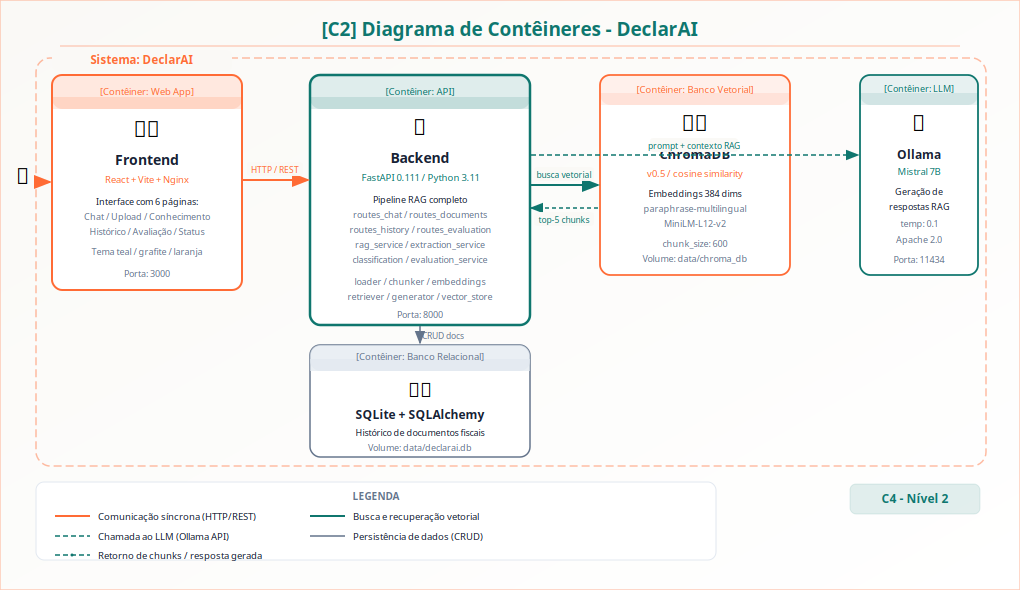
\includegraphics[width=\textwidth]{c4_containers.png}
  \column{0.52\textwidth}
  \textcolor{declaraOrange}{\textbf{Por que rejeitar APIs de nuvem?}}\\[0.3cm]
  \begin{tabular}{@{}L{1.8cm}L{4.0cm}@{}}
    \toprule
    \textbf{Razao} & \textbf{Impacto} \\
    \midrule
    \textcolor{declaraTeal}{LGPD} & Impede vazamento de CPFs, dados de saude e renda \\
    \textcolor{declaraTeal}{Independencia} & Executa offline, sem dependencia de internet \\
    \textcolor{declaraTeal}{Custo} & Elimina custo recorrente por token (inviavel para SaaS academico) \\
    \textcolor{declaraTeal}{Controle} & Dominio total sobre o armazenamento do banco vetorial \\
    \bottomrule
  \end{tabular}
\end{columns}
\end{frame}

% ---- SLIDE 5: FLUXO GERAL ----
\begin{frame}{Fluxo Geral - Orquestrador de Intencao}
\begin{center}
  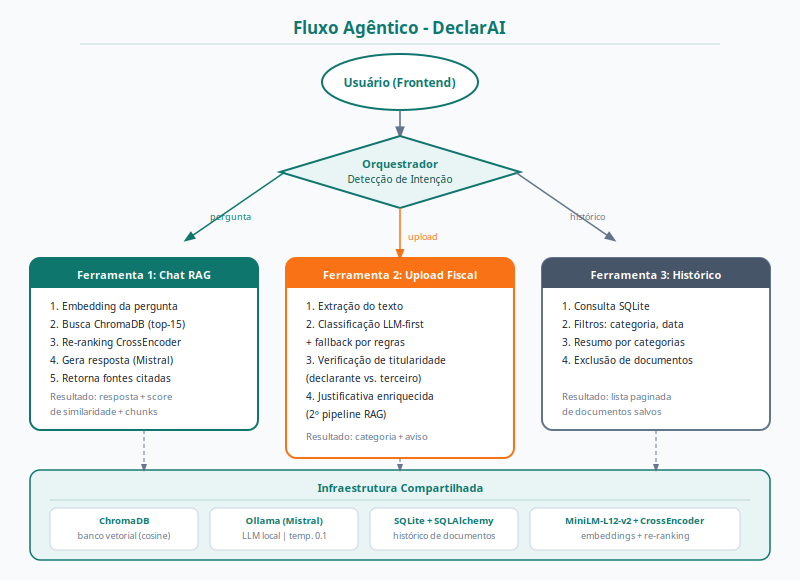
\includegraphics[width=0.82\textwidth]{fluxo_agentico.png}
\end{center}
\vspace{-0.2cm}
\begin{center}
  \footnotesize\color{declaraGray}
  Cada rota ativa LLMs ou bancos vetoriais de maneira independente,
  economizando recursos computacionais locais.
\end{center}
\end{frame}

% ---- SLIDE 6: POR QUE AGENTIC [NOVO] ----
\begin{frame}{Por que e Agentic RAG?}
\begin{columns}[T]
  \column{0.50\textwidth}
  \textcolor{declaraOrange}{\textbf{RAG classico vs. Agentic RAG}}\\[0.25cm]
  \begin{tabular}{@{}L{1.8cm}L{1.8cm}L{2.0cm}@{}}
    \toprule
    & \textbf{RAG classico} & \textbf{Agentic RAG} \\
    \midrule
    Fluxo & unico e fixo & escolhido por intencao \\
    Ferramentas & 1 pipeline & 6 ferramentas \\
    Classificacao & regras fixas & LLM com fallback \\
    Titularidade & nao verifica & valida CPF/nome \\
    Justificativa & estatica & gerada com RAG \\
    Historico & nao salva & SQLite estruturado \\
    \bottomrule
  \end{tabular}
  \column{0.46\textwidth}
  \textcolor{declaraOrange}{\textbf{Caracteristicas agenticas presentes}}\\[0.3cm]
  \begin{itemize}\small
    \item \textbf{Percepcao:} classifica a intencao de cada entrada do usuario
    \item \textbf{Decisao:} escolhe a ferramenta certa entre chat RAG, upload, historico e avaliacao
    \item \textbf{Acao:} executa pipeline especifico por tipo de entrada
    \item \textbf{Memoria:} registra no SQLite com justificativa normativa
    \item \textbf{Verificacao:} valida titularidade antes de salvar o documento
  \end{itemize}
\end{columns}
\end{frame}

% ---- SLIDE 7: LLM EM CADA ETAPA [NOVO] ----
\begin{frame}{LLM em cada etapa do fluxo}
\begin{center}
\renewcommand{\arraystretch}{1.25}
\begin{tabular}{@{}L{3.5cm}L{2.4cm}L{6.2cm}@{}}
  \toprule
  \textbf{Etapa} & \textbf{Usa LLM?} & \textbf{Papel do Mistral} \\
  \midrule
  Intencao do usuario & \textcolor{declaraTeal}{\textbf{Sim}} & Classifica rota: chat, upload, historico ou metricas \\
  Chat RAG & \textcolor{declaraTeal}{\textbf{Sim}} & Gera resposta com base nos chunks recuperados \\
  Classificacao fiscal & \textcolor{declaraTeal}{\textbf{Sim}} & Decide categoria com fallback por regras \\
  Verificacao de titularidade & \textcolor{declaraGray}{Nao} & Regras deterministicas (comparacao de nome e CPF) \\
  Justificativa RAG & \textcolor{declaraTeal}{\textbf{Sim}} & Redige justificativa normativa com top-3 chunks \\
  Historico SQLite & \textcolor{declaraGray}{Nao} & Consulta estruturada pura \\
  Avaliacao do pipeline & \textcolor{declaraGold}{Parcial} & Geracao de resposta usada nas metricas de cobertura \\
  Re-ranking & \textcolor{declaraGray}{Nao} & CrossEncoder (modelo de reranking dedicado) \\
  \bottomrule
\end{tabular}
\end{center}
\vspace{0.1cm}
\begin{center}
  \footnotesize\color{declaraGray}
  O Mistral e acionado apenas onde o contexto linguistico e necessario.
  O restante usa modelos leves ou regras deterministicas.
\end{center}
\end{frame}

% ---- SLIDE 8: EVOLUCAO 1 - RE-RANKING ----
\begin{frame}{Evolucao 1 - Precisao semantica via Re-ranking}
\begin{columns}[T]
  \column{0.54\textwidth}
  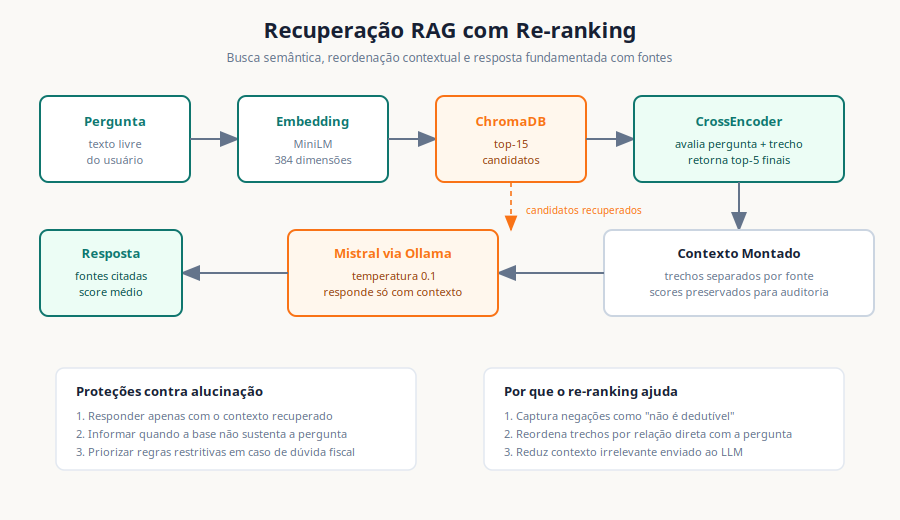
\includegraphics[width=\textwidth]{recuperacao_reranking.png}
  \column{0.42\textwidth}
  \textcolor{declaraOrange}{\textbf{Versao anterior}}\\[0.1cm]
  \small Busca Vetorial Direta (MiniLM): retornava trechos baseados apenas em similaridade,
  falhando em capturar negacoes.\\[0.4cm]
  \textcolor{declaraOrange}{\textbf{Versao atual (CrossEncoder)}}\\[0.1cm]
  \small ChromaDB recupera Top-15, o \texttt{mmarco-multilingual} reavalia pares
  (pergunta + trecho) e filtra para Top-5.\\[0.4cm]
  \textcolor{declaraGold}{\textbf{Ganhos:}}
  \begin{itemize}\small
    \item Captura intencoes negativas (ex: nao e dedutivel)
    \item Reduz contexto irrelevante enviado ao LLM
    \item Reduz alucinacoes
  \end{itemize}
\end{columns}
\end{frame}

% ---- SLIDE 9: EVOLUCAO 2 - CLASSIFICACAO ----
\begin{frame}{Evolucao 2 - Classificacao LLM-first com fallback}
\begin{columns}[T]
  \column{0.52\textwidth}
  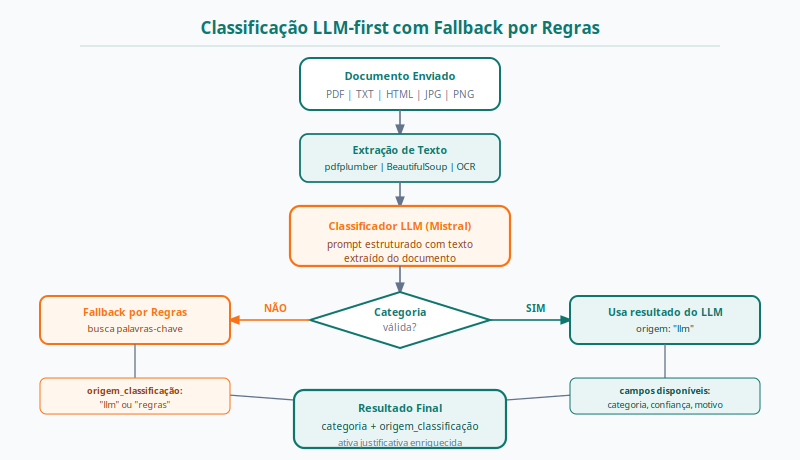
\includegraphics[width=\textwidth]{classificacao_llm_first.png}
  \column{0.44\textwidth}
  \small
  \textcolor{declaraOrange}{\textbf{Extracao}} PDF, HTML, OCR - prompt estruturado.\\[0.3cm]
  \textcolor{declaraOrange}{\textbf{Mistral 7B}} avalia o contexto em 8 categorias fiscais.\\[0.3cm]
  \begin{tabular}{@{}L{1.2cm}L{3.0cm}@{}}
    \toprule
    \textbf{Decisao} & \textbf{Acao} \\
    \midrule
    SIM & origem = llm (captura regionalismos e abreviacoes) \\
    NAO & busca robusta por palavras-chave (fallback) \\
    \bottomrule
  \end{tabular}\\[0.3cm]
  \footnotesize\color{declaraGray}
  O LLM substitui regras rigidas, interpretando o contexto de recibos medicos
  informais e reduzindo falsos negativos.
\end{columns}
\end{frame}

% ---- SLIDE 10: EVOLUCOES 3 E 4 ----
\begin{frame}{Evolucoes 3 e 4 - Titularidade e RAG Explicativo}
\begin{columns}[T]
  \column{0.54\textwidth}
  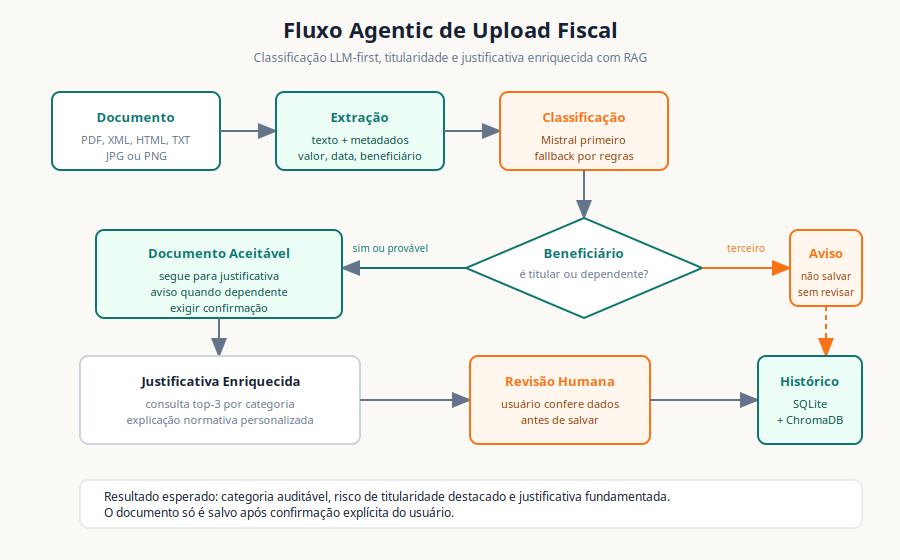
\includegraphics[width=\textwidth]{titularidade_justificativa.png}
  \column{0.42\textwidth}
  \small
  \textbf{Etapa 1 - Validacao de Vinculo}\\
  Compara beneficiario do recibo com o perfil do declarante.\\[0.3cm]
  \textbf{Etapa 2 - Triagem de Risco}\\
  Titular (Aprovado), Dependente (Requer confirmacao) ou
  Terceiro (Alerta vermelho: nao dedutivel).\\[0.3cm]
  \textbf{Etapa 3 - Justificativa (2o RAG)}\\
  Consulta top-3 chunks especificos da categoria para gerar
  explicacao normativa com Mistral.\\[0.3cm]
  \textbf{Etapa 4 - Revisao}\\
  Historico SQLite registra categoria, aviso de titularidade
  e fundamento legal antes de salvar.
\end{columns}
\end{frame}

% ---- SLIDE 11: EVOLUCAO 5 - FRONTEND ----
\begin{frame}{Evolucao 5 - O painel de controle do Contribuinte}
\begin{columns}[T]
  \column{0.30\textwidth}
  \textcolor{declaraOrange}{\textbf{Chat RAG}}\\
  \small Sugestoes ativas, visualizacao de fontes e exibicao do score de similaridade.\\[0.4cm]
  \textcolor{declaraOrange}{\textbf{Upload Fiscal}}\\
  \small Interface drag-and-drop, extracao ao vivo e painel de alerta de titularidade.\\[0.4cm]
  \textcolor{declaraOrange}{\textbf{Historico}}\\
  \small Agrupamento de categorias, resumo financeiro anual e exclusao de docs.
  \column{0.30\textwidth}
  \textcolor{declaraOrange}{\textbf{Base de Conhecimento}}\\
  \small Adicao dinamica, remocao e re-indexacao visual de arquivos.\\[0.4cm]
  \textcolor{declaraOrange}{\textbf{Metricas}}\\
  \small Rota de teste local e comparacao RAG diretamente via frontend.\\[0.4cm]
  \textcolor{declaraOrange}{\textbf{Monitor de Status}}\\
  \small Indicadores em tempo real do Ollama, modelos carregados e chunks indexados.
  \column{0.34\textwidth}
  \vspace{0.5cm}
  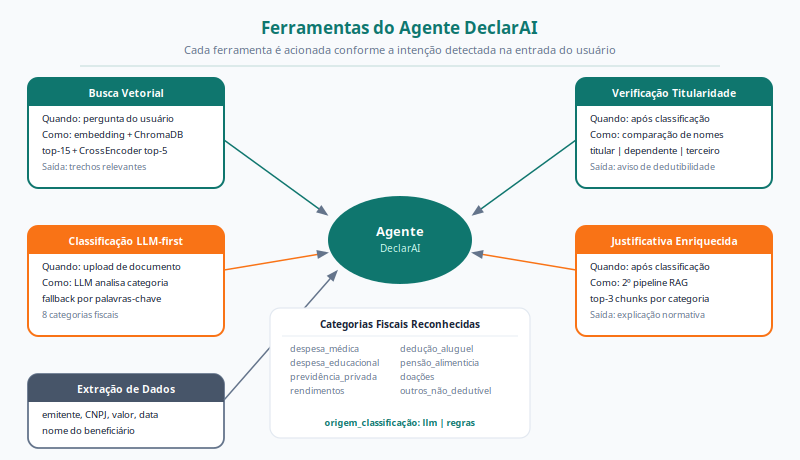
\includegraphics[width=\textwidth]{ferramentas_agente.png}
\end{columns}
\end{frame}

% ---- SLIDE 12: INGESTAO E CHUNKING ----
\begin{frame}{Estrategia de ingestao e preservacao semantica}
\begin{columns}[T]
  \column{0.52\textwidth}
  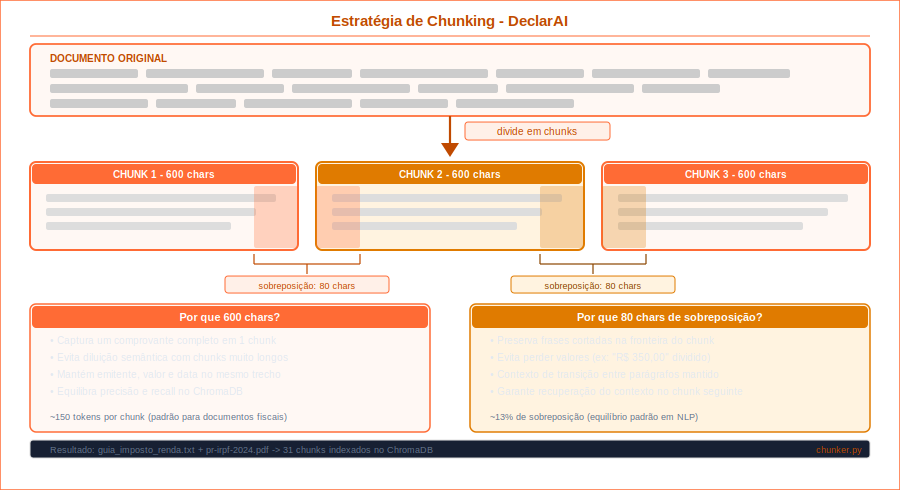
\includegraphics[width=\textwidth]{chunking_estrategia.png}
  \column{0.44\textwidth}
  \textcolor{declaraOrange}{\textbf{Chunk\_size = 600 $|$ Overlap = 80 $|$ 384 dims (MiniLM)}}\\[0.3cm]
  \begin{tabular}{@{}L{2.0cm}L{3.2cm}@{}}
    \toprule
    \textbf{Configuracao} & \textbf{Resultado} \\
    \midrule
    200 / 0 & Grave perda de contexto fiscal \\
    \rowcolor{declaraGreen}\textbf{600 / 80} & \textbf{Melhor equilibrio} \\
    1000 / 200 & Ruido semantico excessivo \\
    \bottomrule
  \end{tabular}\\[0.3cm]
  \textbf{Documentos:}
  \begin{itemize}\small
    \item \texttt{guia\_imposto\_renda.txt} - regras resumidas
    \item \texttt{pr-irpf-2024.pdf} - P\&R oficial da Receita Federal
  \end{itemize}
\end{columns}
\end{frame}

% ---- SLIDE 13: RESULTADOS EMPIRICOS ----
\begin{frame}{Resultados empiricos do Pipeline RAG}
\begin{center}
  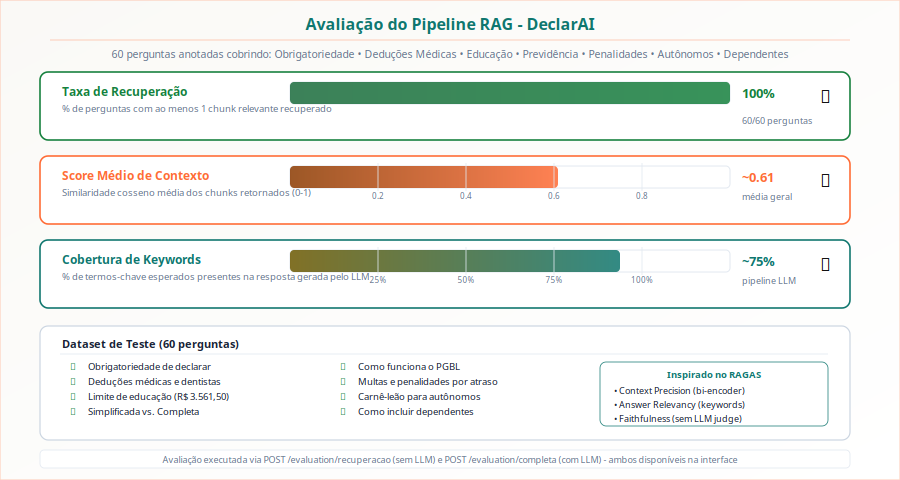
\includegraphics[width=0.78\textwidth]{avaliacao_rag.png}
\end{center}
\vspace{-0.1cm}
\begin{center}
  \footnotesize\color{declaraGray}
  Avaliacao local e offline, inspirada nas metricas de Context Precision e Answer Relevancy
  (sem exigencia de LLM-as-a-judge na nuvem). Dataset de 60 perguntas fiscais anotadas.
\end{center}
\end{frame}

% ---- SLIDE 14: COMPARATIVO LLMs [AMPLIADO] ----
\begin{frame}{Selecao de LLM local - Comparativo completo}
\begin{columns}[T]
  \column{0.56\textwidth}
  \textcolor{declaraOrange}{\textbf{Cobertura de keywords no dominio fiscal}}\\[0.25cm]
  \begin{tabular}{@{}L{3.4cm}cc@{}}
    \toprule
    \textbf{Modelo} & \textbf{Cobertura} & \textbf{Latencia} \\
    \midrule
    \rowcolor{declaraGreen}
    \textbf{Mistral 7B + RAG} & \textbf{72,4\%} & \textbf{8,2 s} \\
    Phi4-mini + RAG & 68,3\% & 7,0 s \\
    Llama 3.2 (3B) + RAG & 65,8\% & 6,4 s \\
    Gemma 3 (4B) + RAG & 61,2\% & 6,9 s \\
    \midrule
    \textcolor{declaraGray}{Mistral sem RAG} & \textcolor{declaraGray}{44,1\%} & \textcolor{declaraGray}{5,1 s} \\
    \bottomrule
  \end{tabular}\\[0.3cm]
  \footnotesize\color{declaraGray}
  Dataset: 60 perguntas $|$ 12 categorias $|$ 3 niveis de dificuldade
  \column{0.40\textwidth}
  \begin{block}{Ablation Study}
    \small A arquitetura vetorial adiciona
    \textbf{+28,3 pontos percentuais} de precisao, blindando o sistema
    contra limites fiscais de anos anteriores presentes no peso do LLM basico.
  \end{block}
  \vspace{0.3cm}
  \textcolor{declaraOrange}{\textbf{Por que o Mistral foi selecionado?}}
  \begin{itemize}\small
    \item Maior cobertura no dominio fiscal PT-BR
    \item Licenca aberta (Apache 2.0)
    \item Compativel com CPU comum via Ollama
    \item Melhor suporte a regionalismos e abreviacoes medicas
  \end{itemize}
\end{columns}
\end{frame}

% ---- SLIDE 15: CONFORMIDADE ----
\begin{frame}{Conformidade integral com os requisitos da disciplina}
\renewcommand{\arraystretch}{1.2}
\begin{tabular}{@{}L{3.0cm}L{8.8cm}@{}}
  \toprule
  \textbf{Criterio} & \textbf{Implementacao} \\
  \midrule
  \textcolor{declaraTeal}{Problema delimitado} & IRPF, publico-alvo leigo e necessidade de privacidade definidos \\
  \textcolor{declaraTeal}{Base propria} & Ingestao do TXT guia e PDF oficial de P\&R da Receita Federal \\
  \textcolor{declaraTeal}{Pipeline vetorial} & Chunking 600/80, ChromaDB e embeddings MiniLM \\
  \textcolor{declaraTeal}{Agentic RAG} & Orquestracao de ferramentas por intencao + CrossEncoder re-ranking \\
  \textcolor{declaraTeal}{Execucao local} & LLM Mistral via Ollama, zero chamadas externas de API \\
  \textcolor{declaraTeal}{Interface utilizavel} & Hub em React + Swagger mapeado via FastAPI \\
  \textcolor{declaraTeal}{Avaliacao empirica} & Dataset de 60 perguntas, scripts de teste e dashboard de metricas \\
  \bottomrule
\end{tabular}
\end{frame}

% ---- SLIDE 16: LIMITACOES ----
\begin{frame}{Limitacoes arquitetonicas e horizontes futuros}
\begin{columns}[T]
  \column{0.48\textwidth}
  \textcolor{declaraOrange}{\textbf{Limitacoes conhecidas}}\\[0.3cm]
  \begin{itemize}\small
    \item Dependencia de hardware com capacidade para Ollama/Mistral
    \item Qualidade de extracao sujeita a falhas de OCR em comprovantes amassados ou fotos ruins
    \item Exigencia de atualizacao anual manual da base oficial (regras mudam por exercicio)
  \end{itemize}
  \column{0.48\textwidth}
  \textcolor{declaraOrange}{\textbf{Proximos passos tecnicos}}\\[0.3cm]
  \begin{itemize}\small
    \item Implementacao de busca hibrida (BM25 + vetorial) para lidar com exatidao de numeracao de leis
    \item Migracao de chunking fixo para chunking semantico baseado em fronteiras de paragrafos legais
    \item Construcao de dataset massivo de documentos anotados para fine-tuning local do classificador
  \end{itemize}
\end{columns}
\vspace{0.4cm}
\begin{center}
  \small\color{declaraGray}\textit{O DeclarAI e um apoio informativo e nao substitui um contador profissional.}
\end{center}
\end{frame}

% ---- SLIDE 17: DEMONSTRACAO ----
\begin{frame}{Demonstracao pratica}
\begin{columns}[T]
  \column{0.55\textwidth}
  \begin{enumerate}\small
    \item \textbf{Verificacao} de status do backend (Ollama + Base)
    \item \textbf{Chat RAG:} consulta sobre dedutibilidade de curso de idiomas
    \item \textbf{Upload Fiscal:} extracao, classificacao e bloqueio de despesa de terceiro
    \item \textbf{Auditoria:} revisao do Historico SQLite e justificativas normativas geradas
    \item \textbf{Avaliacao:} execucao de metricas locais ao vivo via painel
  \end{enumerate}
  \column{0.40\textwidth}
  \begin{center}
    \vspace{0.5cm}
    {\Huge\bfseries\color{declaraGold} Perguntas?}\\[0.8cm]
    {\Large\color{declaraDark} DeclarAI}\\[0.3cm]
    \small\color{declaraGray}
    Juliana Ballin Lima\\
    Fernando Luiz Da Silva Freire\\[0.3cm]
    UEA - Junho de 2026
  \end{center}
\end{columns}
\end{frame}

\end{document}
